%; whizzy chapter -dvi
% -initex iniptex -latex platex -format platex -bibtex jbibtex -fmt fmt
% 以上 whizzytex を使用する場合の設定。
 
%     Tokyo Debian Meeting resources
%     Copyright (C) 2012 Junichi Uekawa
%     Copyright (C) 2011, 2015 Nobuhiro Iwamatsu

%     This program is free software; you can redistribute it and/or modify
%     it under the terms of the GNU General Public License as published by
%     the Free Software Foundation; either version 2 of the License, or
%     (at your option) any later version.

%     This program is distributed in the hope that it will be useful,
%     but WITHOUT ANY WARRANTY; without even the implied warranty of
%     MERCHANTABILITY or FITNESS FOR A PARTICULAR PURPOSE.  See the
%     GNU General Public License for more details.

%     You should have received a copy of the GNU General Public License
%     along with this program; if not, write to the Free Software
%     Foundation, Inc., 51 Franklin St, Fifth Floor, Boston, MA  02110-1301 USA

%  preview (shell-command (concat "evince " (replace-regexp-in-string "tex$" "pdf"(buffer-file-name)) "&"))

%%ここからヘッダ開始。

\documentclass[mingoth,a4paper]{jsarticle}
\usepackage{monthlyreport}
% 日付を定義する、毎月変わります。
\newcommand{\debmtgyear}{2016}
\newcommand{\debmtgmonth}{6}
\newcommand{\debmtgdate}{25}
% started from zero:
% (let ((year 2013) (month 7)) (+ (* (- year 2005) 12) month -1))
\newcommand{\debmtgnumber}{140}

% コードハイライトの為の設定
\makeatletter\chardef\pdf@shellescape=\@ne\makeatother
\usepackage{minted}

\begin{document}

\begin{titlepage}
\thispagestyle{empty}
% タイトルページ:編集必要な部分は最初のマクロに飛ばすこと

\vspace*{-2cm}
第\debmtgnumber{}回 東京エリア Debian 勉強会資料\\
\hspace*{-2cm}

\includegraphics{image2012-natsu/dotdeb.pdf}\\
\hfill{}\debmtgyear{}年\debmtgmonth{}月\debmtgdate{}日

% ここはアップデートすること
% 全角文字にしないとフォントのサイズが合わないので注意
\rotatebox{10}{\fontsize{30}{30} {\gt 特集 :debexpo(mentors.d.n)をハックするには}}\\

\vspace*{-2cm}
\hfill{}
\includegraphics[height=6cm]{image200502/openlogo-nd.eps}
\end{titlepage}

\newpage

\begin{minipage}[b]{0.2\hsize}
 \definecolor{titleback}{gray}{0.9}
 \colorbox{titleback}{\rotatebox{90}{\fontsize{80}{80} {\gt デビアン勉強会} }}
\end{minipage}
\begin{minipage}[b]{0.8\hsize}
\hrule
\vspace{2mm}
\hrule
\begin{multicols}{2}
\tableofcontents
\end{multicols}
\vspace{2mm}
\hrule
\end{minipage}

%\dancersection{事前課題}{杉本 典充}
%
%今回の事前課題は以下です:
%\begin{enumerate}
%\item q1
%\item Hack Timeは何をしますか。
%\end{enumerate}
%この課題に対して提出いただいた内容は以下です。
%\begin{multicols}{2}
%{\small
%\begin{prework}{ ����(yy\_y\_ja\_jp) }
���ޤ���������ǤϤʤ��Ǥ���... �긵�Υ�åץȥåפǤ� /boot �ˤ� ext2
 ����¾�ˤ� ext3���Ƕ�ȤäƤ���ǥ����ȥåפǤ� /boot �ˤ� ext3 ����¾
 �ˤ� LVM ��� ext4 ��ȤäƤ��ޤ���
\end{prework}

\begin{prework}{ �����ϥ� }
�ǥե���Ȥ�ext3����
�����ǥե���ȤΤޤޡ�
(NTFS���VM���᡼�����ext3�⤢�뤱��)
\end{prework}

\begin{prework}{ yos.takahashi }
ext3/4���˻ȤäƤޤ���ext3�Υǡ�������١����ˤĤ�������Linux2011ǯ1���˼�ɮ���ޤ�����
\end{prework}

\begin{prework}{ MATOHARA }
����inode �ϳ���������Ƥ���inode ��ưŪ�˳�����Ƥ���XFS �����򤹤뤳
 �Ȥ�¿���Ǥ���NILFS �Ͼ�����Ƥߤ��ΤǤ�����mount ���˰ʲ��Τ褦�ʥ��
 ���������ФƤޤ��ݤ��ʤȻפ��ޤ�����
\begin{commandline}
$ sudo mount /dev/sdb1 /mnt
mount.nilfs2: WARNING! - The NILFS on-disk format may change at any time.
mount.nilfs2: WARNING! - Do not place critical data on a NILFS filesystem. 
\end{commandline}
����¾NotePC �Ǥ�dm-crypt �ξ�˥ե����륷���ƥ���֤��ưŹ沽�����ꡢ
 eCryptfs �ǰŹ沽�����ꤷ�Ƥ��ޤ����񤭹��߻���CPU �򤫤ʤ���񤷤ޤ��ġ�
\end{prework}

\begin{prework}{ ��ޤ� }
��ext2-$>$reiserfs-$>$jfs-$>$xfs-$>$reiserfs-$>$ext3�ȻȤäƤ��ޤ�����

����:
\begin{itemize}
 \item reiserfs: ���ե������¿���ե�����Υ������������ӥ��Ӥ��Ƥ��ɤ���
       �����������դȤ����ⵤ�������θ�μ�žȬ�ݥ����ɤˡ�����
 \item jfs: ����v1.0��̾��ä�IBM���ꥨ�ʥ��������ˤ�xfs��ƨ��
 \item xfs: fsck==true�˴�ư����������ǯ�Ȥä���ΤΥޥ�����Ĵ����0byte
       �ե��������������Ѥ���줺ƨ����
\end{itemize}
������reiser4��Ķ���Ԥ��뤦���ˤ��줬�����ʤäơ����ext3�˸��경��htree�����ä������⤦Ŵ�Ĥʤ鲿�Ǥ⤤���Ǥ��������Ȥ����Ĥ�nilfs�ʤɤ˼��Ф��Ƥ��ޤ���ext3�������noatime���٤Ǥ����������aufs���碌�Ƽ�ʬ���Ȥ��Ȥ� *strap �Ķ��򥯥����˥󥰤��Ƥ��ޤ����¸����ƥ��Ȥ������Ǥ�����Ǥ���USB�����ư�Ǥ�ͭ�ѡ�

���LVM�ǤϤʤ�MD��Ȥäƾ�Ĺ���ܥХå����åפ򤷤Ƥ��ޤ���
 MD(sda,sdb,sdc)�ǹ��ۤ����̾��MD(����)�Dz�ư���Хå����åפλ���
 attach/detach�򤹤롣�֥��å���٥�ʤΤǥꥫ�Х��FSǤ���Ǥ��������̤�
 �������¾����ˡ���ʤ�������
\end{prework}

\begin{prework}{ henrich }
�ȤäƤ���֤�NTFS��Ĺ���󤸤�ʤ��Ǥ����͡����졣
�����Ρ����Ѥο������ǥ�������ext4�ǥե����ޥåȤ��ޤ����������㤤��Ƚ��ʤ��Ȥ����������Ƥ��ޤ���
\end{prework}

\begin{prework}{ emasaka }
�Ĥ뤷��FS��ȤäƤޤ�
\end{prework}

\begin{prework}{ �ܾ� }
ext3����Ѥ��Ƥ��ޤ����ä��Ѥ�ä����ȤϤ��Ƥ��ޤ���
FS����ʤ��Ǥ������Ƕ�Lenny��2TB��HDD��Ȥä���parted�äƤλȤ��ƶä��ޤ�����
\end{prework}

\begin{prework}{ ����@������ }
���������Ū�˳��Ѥ��Ƥ���ե����륷���ƥ��ReiserFS�Ǥ���
�Ż��ǻȤäƤ�Ķ���ext3�Ǥ�����ext3���Ÿ������ǥ��㡼�ʥ뤬
����Ʋ��Ǥ������ηи��ʸŤ������ͥ�Ǥ���...�ˤ����ꡢ
���ޤ꿮�Ѥ��Ƥ��ޤ���
�����ReiserFS�Ķ��ǤϤ���ޤǤνꤤ���ʤ��Ÿ����ڤä��ꡢ
�Ƥ�HDD�����줫�����ꤷ�Ƥ��ﳲ����ä��и���̵���Τǡ�
��³Ū�˻ȤäƤ��ޤ���
��ǯ����ReiserFS�Υᥤ��ȯ��(Hans Reiser)�����ᤵ��Ƥ��ޤ������ƥʥ󥹤��ۤ��Ƥ��ޤ�����
�����������θ��ReiserFS��¾�γ�ȯ�Ԥˤ���³�����ݼ餵��Ƥ���Τǡ��¿����ޤ�����
\end{prework}

\begin{prework}{ nozzy123nozzy }
\begin{enumerate}
 \item LVM�ˤĤ��Ƥϡ�CentOS5.5��Ƴ�������Τ��Τޤޤ����Ѥ��Ƥޤ�����
       ���������ƥब��äƤ���Volume̾�ϥǥե���Ȥ�����ȡʼºݤˤ�
       kickstart�ˤơˤ��ѹ����ƻȤäƤޤ����ʾ㳲���Υ���١����˺��뤿
       ���
\item ext3�ˤĤ��Ƥϡ�debian-sid�����Τޤ޻��ꤷ�Ƥ����Τ򤽤Τޤ޻Ȥ�
      �Ƥ����ꤷ�ޤ���relatime, noatime ���餤�Ͼ����ɲä��Ƥߤ����ʡ���
      �ϻפäƤޤ���
\end{enumerate}
\end{prework}

\begin{prework}{ �ޤ��������ؤ� }
\begin{itemize}
 \item Debian�Ǥ��ä˶Ťä����Ȥ�����ext3��ȤäƤޤ������ۥޥ����qcow2
       ���᡼���ǥ��������ѻ��ʳ��ϡ�LVM�ϻȤäƤޤ���
 \item �����ǰ����ü�ʤΤϡ��������DHCP�������Ѥ�Armadillo-J�ǻȤäƤ�
       ��JFFS�Ǥ����ǥե���ȤΥե����०�����Ǥϥ�֡��Ȥ�����������
       �ƽ��������Ƥ��ޤ��Τǡ�RAM�ΰ�˽񤭤��ߡ��Ÿ��ڤäƤ�ä��ʤ�
       ���������Ǥ���Debian��udhcp�Υ������ѥå���������ӥ�ɤ��ƻȤäƤޤ���
       \footnote{\url{http://d.hatena.ne.jp/mkouhei/20080601/1212330630}}
 \item ��Debian���ߤǡ���ʬ����ǰ��֥ۥåȤʤΤ�palm webOS�Ǥ��������Ubuntu��
       �������ޥ���������Τ餷���ΤǤ�����/etc/mtab�򸫤��35�Ԥ⤢�ꡢ
       ���ʤ����֤ʹ����Ǥ��͡�
\end{itemize}
\end{prework}
%}
%\end{multicols}

\dancersection{Debian Trivia Quiz}{杉本 典充}

Debianの昨今の話題についてのQuizです。

今回の出題範囲は\url{debian-devel-announce@lists.debian.org} や \url{debian-news@lists.debian.org}に投稿された内容などからです。

\begin{multicols}{2}
%; whizzy-master ../debianmeetingresume201311.tex
% $B0J>e$N@_Dj$r$7$F$$$k$?$a!"$3$N%U%!%$%k$G(B M-x whizzytex $B$9$k$H!"(Bwhizzytex$B$,MxMQ$G$-$^$9!#(B
%

\santaku
{stable$BHG$N(Bjessie$B$G$bDs6!$,3+;O$5$l$?(Biceweasel$B$N%"%C%W%G!<%H!#%Q%C%1!<%8L>$,JQ$o$C$F$$$^$9!#2?$K$J$C$?$G$7$g$&$+(B}
{iceweasel-esr}
{firefox}
{firefox-esr}
{firefox-esr}
{$B%j!<%,%kLdBj$,$R$HCJMn$7!"(Bdebian$B$G$b(Bfirefox$B$H$7$FDs6!$G$-$k$3$H$K$J$j$^$7$?!#=>Mh$N(Bjessie$B$G$O(Biceweasel ver38esr$B$,Ds6!$5$l$F$$$^$7$?!#:#2s$O(Bfirefox-esr$B%Q%C%1!<%8$H$7$F(Bver45esr$B$NDs6!$,3+;O$5$l$^$7$?!#(B}

\santaku
{Debian Administrator$B!G(Bs Hanbook(Debian$B4IM}<T%O%s%I%V%C%/(B)$B$H$$$&%I%-%e%a%s%H$,$"$j$^$9!#KDBg$JNL$N%I%-%e%a%s%H$G$"$j$^$9$,!"$D$$$KF|K\8lHG$,%j%j!<%9$5$l$^$7$?!#K]Lu:n6H$KB?Bg$J9W8%$r$7$F$$$?$@$$$?J}$OC/$G$7$g$&$+!#(B}
{Ryuunosuke Ayanokouzi}
{Norimitsu Sugimoto}
{Hideki Yamane}
{Ryuunosuke Ayanokouzi}
{Debian$B4IM}<T%O%s%I%V%C%/$OL5NA$N(Bweb$BHG5Z$SEE;R=q@RHG!"M-NA$N=q@RHG$,$"$j$^$9!#:#8e$NK]Lu:n6H7QB3$N$?$a$K4sIU$rJg$C$F$$$^$9!#$J$*!"%j%j!<%9%"%J%&%s%9$N%Z!<%8$O<!$N(BURL$B$O<!$NDL$j$G$9!#(B\url{https://debian-handbook.info/2016/get-the-japanese-version-of-the-debian-administrators-handbook/}}

\end{multicols}


\dancersection{最近のDebian関連のミーティング報告}{杉本 典充}

\subsection{第139回東京エリアDebian勉強会}

2016年5月21日(土)に第139回東京エリアDebian勉強会を開催しました。会場は銀座にある朝日ネットさんをお借りして行いました。参加者10名でした。

発表者はRogerさんで、表題は「Buffalo Linkstation向けDebian InstallerDebian Installer」という内容でした。

RogerさんはLinkstationへDebian GNU/Linuxをインストールして利用できるようにハックしている方です。発表ではARMデバイス上でDebian Installerを実行する仕組みを解説していただき、実際にLinkstationへDebian GNU/Linuxをインストールするデモを実施しました。ARMデバイスへDebianをインストールする作業はDebian Installerを利用しない場合も多いため、参加者も初めて見る方が多かったようです。また、Linkstationをハックした成果である実行コマンドのチューニングパラメータに関する質問もありました。

発表終了後は、各自の課題をこなす作業時間としました。

% % (query-replace-regexp "<.*?>" "")
% % (query-replace-regexp "^[	 ]\+" "")

%-------------------------------------------------------------------------------
\dancersection{debexpo(mentors.d.n)をハックするには}{林健太郎(kenhys)}
%-------------------------------------------------------------------------------

\subsection{はじめに}

そのへんに生えているDebian使いがDebian公式パッケージを更新するにあたっては、更新したパッケージをDebian開発者にスポンサーしてもらう必要があります。

その際のパッケージのアップロード先には、mentors.debian.netというWebサイトがよく使われています。

今回はmentors.debian.netをハックする機会があったので、その内容を紹介します。\footnote{2016年8月現在の情報で、現在では若干記述が古くなっている箇所があります。該当箇所には注記を入れてあります。}

\subsection{debexpoとは?}

http://mentors.debian.net(以下mentors.d.n)を支えるウェブアプリケーションのことです。リポジトリ名がdebexpoになっています。

\begin{center}
\includegraphics[width=0.5\hsize]{image201606/mentors.d.n.eps}
\end{center}

debexpoの公式サイトは\url{https://alioth.debian.org/projects/debexpo/}です。
以前開発の中心となっていたサイト\url{https://workaround.org/project/debexpo}にはdebexpoの名前の由来が次のように記載されています。

\begin{quotation}
The new project was called "debexpo" because it was supposed to become an {\color{red}expo}sition for {\color{red}Deb}ian packages.
\end{quotation}

パッケージが一同に会する展覧会とでもいったところでしょうか。

\subsubsection{debexpo概要}

debexpoの位置付けがどういうものかなんとなくわかったところで、もうすこし具体的な紹介をしましょう。

debexpoの特徴をいくつか紹介すると以下があげられます。

\begin{itemize}
\item Python製
\item Pylons\footnote{\url{http://www.pylonsproject.org/}}フレームワーク採用
\item テンプレートエンジンはMako\footnote{\url{}}
\end{itemize}

このPylonsというフレームワーク、あまり知らない人がいるかも知れませんので補足しておくと、

\begin{itemize}
\item Railsっぽいフレームワーク
\item 2011年にメンテナンスモード入りした枯れたフレームワークです
\item 後継としてPyramidというフレームワークが開発されています
\end{itemize}

という特徴があります。

\begin{itembox}[l]{コラム:debexpoにもゆるキャラが?}
\includegraphics[width=0.2\hsize]{image201606/debexpo-mascot-zoom.eps}
debexpoには、実はゆるキャラが設定されています。Webサイトの左上隅の赤枠で囲っているところに何かいますよね、それです。
ただし、詳細は不明です。SUUMO\footnote{不動産情報サイト。\url{http://suumo.jp/}}のスーモ\footnote{マスコットキャラクター。スーモの部屋\url{http://suumo.jp/edit/suumo-heya/}という特設ページがある。}には片思いのスモミとの想像上の子供スモルがいるという設定\footnote{\url{http://suumo.jp/edit/suumo-heya/character/suumo_character.pdf}}
があるくらいなので、このキャラにも何かありそうな気もしますが。。。
\end{itembox}

\subsection{なぜdebexpoをハックする必要が?}

パッケージをスポンサーしてもらうときに使うmentors.d.nにはいくつかお薦めな点があります。

\begin{itemize}
  \item パッケージのチェックもしてくれる
  \item RFSのテンプレートも生成してくれる
\end{itemize}

\begin{screen}
  \includegraphics[width=0.8\hsize]{image201606/qa-information.eps}
\end{screen}

スクリーンショットからもわかるように、QA informationの欄にLintianの警告などが表示されるようになっています。

\begin{screen}
  \includegraphics[width=0.5\hsize]{image201606/view-rfs-template.eps}
\end{screen}

また、スクリーンショットの「View RFS template」のリンクをたどると、RFSのテンプレートも生成してくれるというのも嬉しいポイントです。

なので、あとはこのRFSテンプレートをもとにして、メールするだけになっています。\footnote{とはいうものの、嘘ではないが、正確でもない。}

実際のRFS templateを見てみましょう。

\begin{screen}
\includegraphics[width=0.5\hsize]{image201606/rfs-template-pithole.eps}
\end{screen}

[fill in]の文字がちらほらあるのがわかりますね。

\begin{screen}
\includegraphics[width=0.5\hsize]{image201606/rfs-template-pithole2.eps}
\end{screen}

これだけではありません。ほかにも穴埋めが必要です。

\begin{screen}
\includegraphics[width=0.5\hsize]{image201606/rfs-template-fill-in1.eps}
\end{screen}

Subject:に種別を書かないといけません。

\begin{screen}
\includegraphics[width=0.5\hsize]{image201606/rfs-template-fill-in2.eps}
\end{screen}

Severity:を書かないといけません。

\begin{screen}
\includegraphics[width=0.5\hsize]{image201606/rfs-template-fill-in3.eps}
\end{screen}

Upstream,URL,License:を書かないといけません。

\begin{screen}
\includegraphics[width=0.5\hsize]{image201606/rfs-template-fill-in4.eps}
\end{screen}

Changelogを書かないといけません。

これで終わりでしょうか。いいえ違います。

\begin{screen}
\includegraphics[width=0.5\hsize]{image201606/rfs-template-fill-in5.eps}
\end{screen}

さりげなく埋めこまれたhelloとexample.comが残っています。

ようやくあれこれ直し終えました。これでメールが出せると、思うかも知れません。事実私も最初はそう思いました。

ここで問題になるのが、先頭に埋めこまれたスペース2つです。

\begin{screen}
\includegraphics[width=0.5\hsize]{image201606/rfs-template-pithole3.eps}
\end{screen}

ここで、上記はコマンドメールであることを思いださねばなりません。つまり、そのままメールするともちろんエラーになります。

したがって、「なぜdebexpoをハックするのか?」に対する答えは、「RFSテンプレートの残念っぷりをどうにかしたい」から、ということになります。

\begin{screen}
\includegraphics[width=1.0\hsize]{image201606/alioth-debexpo-313593-request.eps}
\end{screen}

Aliothをみてみると、同じ思いの人がいました。それはAliothのtrackerで4年も前に通った道だ、という。

\subsection{どうやってハックしたのか?}

おおむね、以下の流れでdebexpoをハックすることになりました。

\begin{itemize}
  \item upstream探し
  \item ドキュメント探し
  \item まずは動かしてみる
  \item あたりをつけて修正
  \item そしてPRへ
\end{itemize}

特別なことは何もなくて、よくあるフリーソフトウェアの修正です。

\begin{itembox}[l]{コラム:debexpoの歴史について}
debexpoは2003年に最初のコードがPerlで書かれました。しかし、機能拡張の要望に応えたりしていくには支障があったため、Pythonで書き直されたという経緯があります。
debexpoの開発が活発になったのは、2008年のことです。Google SoCに採択されたため、Jonny Lamb氏らにより一気に開発がすすみました。

2009年から2010年はゆるやかな開発が続きました。http://expo.debian.net/が公開されたのもこのころです。現在のmentors.d.nへと切り替えられたのは2011年のことです。
その後も、2012年にはUIの改善(debexpo v2)や再度GSoCへの採択(debexpo v3)などと開発が続いています。

このあたりの変遷について、Nicolas Dandrimont氏による「The State of mentors.debian.net GSOC and Beyond」という発表資料に詳しく書かれているので興味がある人は参照するとよいでしょう。
\footnote{\url{http://fr2012.mini.debconf.org/slides/debexpo.pdf}}
\end{itembox}

\subsubsection{upstream探し}

\begin{screen}
\includegraphics[width=0.5\hsize]{image201606/source-code-and-bugs.eps}
\end{screen}

debexpoの場合には、mentors.d.n下部にリンクがきちんとあるので、Aliothをみればいいとわかりました。

\begin{screen}
\includegraphics[width=0.5\hsize]{image201606/last-change-on-alioth.eps}
\end{screen}

ただ、どうやら最近はコミットがないのが不安になりました。
よく使われているならそこそこメンテされているイメージがあったからです。実際にはそうでもありませんでした。

\begin{screen}
\includegraphics[width=0.7\hsize]{image201606/last-change-on-github.eps}
\end{screen}

あとから、GitHubのほうが実は新しい\footnote{\url{https://github.com/debexpo/debexpo}}ことがわかりました。

実際の運用としては、Aliothがmaster\url{https://alioth.debian.org/projects/debexpo/}で、GitHubのをマージという運用になっているようです。

\subsubsection{ドキュメント探し}

リポジトリのdocs/*にドキュメントが整備されていました。インストール手順はdocs/installing.rstを参照すればよいとわかりました。
ただ、残念なことにその内容の一部はリンク先が404になってしまっていました。

\subsubsection{まずは動かしてみる}

ドキュメントから、セットアップ方法は3種類あることがわかりました。

\begin{itemize}
  \item 既存システムにインストール
  \item virtualenvでインストール
  \item VirtualBoxでインストール
\end{itemize}

まずはVirtualBoxで試してみることにしました。環境を分けたいのがその選択理由です。
ただ、Vagrantfileがアレな状態であることがわかりました。

\begin{screen}
\begin{minted}{sh}
# Every Vagrant virtual environment requires a box to build off of.
config.vm.box = "chef/debian-7.6"
\end{minted}
\end{screen}

Debian 7.6 (2014年7月12日)?になっていました。Debian 7.10がもうすでにでているご時世にも関わらずです。

vagrant upしてみるとまた残念な状態でした。

\begin{commandline}
$ vagrant up
Bringing machine 'default' up with 'virtualbox' provider...
==> default: Box 'chef/debian-7.6' could not be found. Attempting to find and install...
  default: Box Provider: virtualbox
  default: Box Version: >= 0
The box 'chef/debian-7.6' could not be found or
could not be accessed in the remote catalog. If this is a private
box on HashiCorp's Atlas, please verify you're logged in via
`vagrant login`. Also, please double-check the name. The expanded
URL and error message are shown below:

URL: ["https://atlas.hashicorp.com/chef/debian-7.6"]
Error: The requested URL returned error: 404 Not Found
}
\end{commandline}

boxが見つからなくてコケていました。そこで、PR\#32で修正しました。
失敗していたのは、Bento projectに移行していたせいでした。

\begin{screen}
\includegraphics[width=0.7\hsize]{image201606/debexpo-pr32-use-latest-wheezy.eps}
\end{screen}

起動して、ログインするには次のようにします。

\begin{commandline}
$ vagrant up --provision
$ vagrant ssh
\end{commandline}

vagrant sshしてpasterコマンドを実行してサーバーを起動します。

\begin{commandline}
$ cd debexpo
$ . venv/bin/activate
$ paster serve development.ini
\end{commandline}

このようにすると、5000ポートでサーバーを起動することができます。

\begin{screen}
\includegraphics[width=0.5\hsize]{image201606/debexpo-on-localhost.eps}
\end{screen}

これによりブラウザでアクセス可能になります。

次にユーザーの追加をします。方法は2つあって、ブラウザ経由で追加するのと、JSONをもとに追加するやりかたがあります。

\begin{screen}

\includegraphics[width=0.5\hsize]{image201606/debexpo-sign-me-up.eps}
\end{screen}

JSONで追加するなら次のような内容のファイルを用意します。

\begin{screen}
\begin{minted}{javascript}
{
  "realname":"Hayashi Kentaro",
  "password":"password",
  "email":"hayashi@clear-code.com"
}
\end{minted}
\end{screen}

ユーザー追加用のスクリプトが用意されているので、それを利用します。

\begin{commandline}
$ python ./bin/user_importer.py -i development.ini -u user.json
\end{commandline}

次にアカウントの有効化をします。アカウントを有効にするには2つ設定をする必要があります。

\begin{itemize}
\item verification (ログインに必要)
\item dmup (アップロードに必要)
\end{itemize}

verificationの設定は次のようなクエリを実行することで行います。

\begin{screen}

\includegraphics[width=0.7\hsize]{image201606/update-verification.eps}
\end{screen}

verificationを空にすることで、メールによる確認プロセスを迂回することができます。

もう一つ、DMUPとはマシン使用ポリシーのことです。開発で使うだけなので、次のようなクエリを実行することでdmupフィールドを更新して、同意したことにします。

\begin{screen}

\includegraphics[width=0.7\hsize]{image201606/update-dmup.eps}
\end{screen}


ここまでできたら、あとはアップロードするために、.dput.cfの設定をします。

\begin{screen}
\begin{minted}{sh}
[debexpo]
fqdn = localhost:5000
incoming = /upload/kenhys@gmail.com/password
method = http
allow_unsigned_uploads = 0
\end{minted}
\end{screen}

用意できたら、実際にアップロードを試してみましょう。

\begin{commandline}
Uploading to debexpo (via http to localhost:5000):
Uploading groonga_6.0.2-1.dsc:
Upload failed: 500 Internal Server Error
\end{commandline}

と思ったら、あっさり500 Internal Server Errorに遭遇しました。

\begin{screen}

\includegraphics[width=0.7\hsize]{image201606/find-a-debexpo-bug.eps}
\end{screen}

残念なことに、あるべきディレクトリがないというオチでした。

そこで、PR\#34で修正してとりこんでもらいました。

\begin{screen}
\includegraphics[width=0.7\hsize]{image201606/debexpo-pr34-incoming-directory.eps}
\end{screen}

PRを出してみたときに気づいたのですが、最後にテストが通ったの8ヶ月前というオチがついていました。

\begin{screen}
\includegraphics[width=0.7\hsize]{image201606/broken-ci-since-8month-ago.eps}
\end{screen}

これはなぜかというとTravis-CIの環境の変化に誰も気いていない状態だったためです。しばらくコミットがなされていないプロジェクトではありがちです。
そこで、PR\#38でテストが通るように修正しました。

\begin{screen}
\includegraphics[width=0.7\hsize]{image201606/debexpo-pr38-broken-ci.eps}
\end{screen}

また、Python2.6でCIはもう不要なので、PR\#37で修正も行いました。

\begin{screen}
\includegraphics[width=0.7\hsize]{image201606/debexpo-pr37-drop-py26.eps}
\end{screen}

ここまで修正して、ようやくパッケージを取り込むところまでたどりつきました。パッケージの取り込みは次のコマンドを実行します。

\begin{commandline}
$ ./bin/debexpo_importer.py \
  -c /tmp/debexpo/growl-for-linux_0.8.5-1_source.changes -i development.ini --skip-gpg-check --skip-email
\end{commandline}

インポートスクリプトを実行したら、あっさり取り込みできずにトレースを吐きました。

\begin{commandline}
Traceback (most recent call last):
  File "./bin/debexpo_importer.py", line 60, in
  i.main()
  File "/home/vagrant/debexpo/debexpo/importer/importer.py", line 473, in main
  gpg = get_gnupg()
  File "/home/vagrant/debexpo/debexpo/lib/utils.py", line 119, in get_gnupg
  return gnupg.GnuPG(config['debexpo.gpg_path'],
  File "/home/vagrant/debexpo/venv/local/lib/python2.7/site-packages/paste/registry.py", line 146, in getitem
  return self._current_obj()[key]
  KeyError: 'debexpo.gpg_path'
\end{commandline}

gpgの検証をスキップするオプションが期待するように動作していなかったので、オプションを正しく解釈するように PR\#39で修正しました。

\begin{screen}
\includegraphics[width=0.7\hsize]{image201606/debexpo-pr39-skip-gpg.eps}
\end{screen}

これでようやく、取り込んだパッケージをWebの画面から確認することができるようになりました。

\begin{screen}
\includegraphics[width=0.7\hsize]{image201606/debexpo-package-list.eps}
\end{screen}

\subsubsection{あたりをつけて修正}

パッケージをアップロードして、画面から確認できるようになったので、次に本来やりたかったdebexpo自体の改善に取り組みました。
まずはディレクトリ構成からあたりをつけることにしました。

\begin{commandline}
config
controllers
cronjobs
importer
i18n
lib
model
plugins
public
templates
tests
\end{commandline}

手がかりとなるのはURLです。

\begin{screen}
\includegraphics[width=0.7\hsize]{image201606/debexpo-investigate-rfs-template-link.eps}
\end{screen}

知りたいのはView RFS Templateのリンク先です。

\begin{screen}
http://localhost:5000/sponsors/rfs-howto/xxxx
\end{screen}

リンク先がわかったので、対応するルーティングを処理するコントローラの実装を探してみたらcontrollers/sponsor.pyを見ればいいことがわかりました。

\begin{screen}
\begin{minted}{python}
def rfs_howto(self, packagename = None):
    c.package = None
    c.package_dir = None
    if packagename:
        package = meta.session.query(Package)
                    .filter_by(name=packagename).first()
        if package:
            c.package = package
            c.package_dir = get_package_dir(package.name)

    return render('/sponsor/rfs_howto.mako')
\end{minted}
\end{screen}

これに対応するMakoのテンプレートはtemplates/sponsor/rfs\_howto.makoにあることがわかりました。
なんとなく見覚えがありますね。

\begin{screen}
\begin{minted}{sh}
    Package: sponsorship-requests
    Severity: normal [important for RC bugs, wishlist for new packages]

    Dear mentors,

    %if c.package:
      I am looking for a sponsor for my package "${ c.package.name }"
    %else:
      I am looking for a sponsor for my package "hello":
    %endif
\end{minted}
\end{screen}


やりたいことは、RFSテンプレートから[fill in]を撲滅し、mailto:リンクを生成してRFSを出すときの手間を軽減することです。
当初の目論見では、\${ c.package.name }とかあるので、テンプレートを書き換えればいいだけかと思っていました。
しかし、結論からいうとこの案は無理でした。というのも、必要なメタ情報を保持していないことが明らかになったからです。持ってないものは表示できません。そのため、どうにかして情報をかき集めないといけないことになりました。

\subsubsection{収集するにはどうすればいいか}

まずは、インポートの処理の流れを把握する必要があります。そして、どのタイミングで収集すべきかを知らなければなりません。また不足している情報は何かを知る必要もあります。

では、実際のインポート処理はどのようになっているのでしょうか。

インポート処理は、dputでmentors.d.nへアップロードされた時点で始まります。そして、前処理が実行され、パッケージのインポート処理へと続いていきます。
もう少し詳しく説明すると、dputしたファイルは/tmp/debexpo/pubへ保存されます。そして、インポート前処理で/tmp/debexpoヘ移動されます。このとき、orig.tar.gzがなかったりするとrejectメールが送られます。

インポートが完了した時点で、ソースパッケージは/tmp/debexpo/filesへと移動されています。このとき、/tmp/debexpo/files以下にはpoolやdist,gitディレクトリが作成されます。
また、各種パッケージの情報がインポート中にデータベースへと保存されるようになっています。

\subsubsection{収集すべきデータを確認する}

収集するべきデータを確定するには、メタ情報がどのように保持されているのかを把握する必要があります。そこで実際のテーブルを覗いてみることにしました。
debexpoで使用している主なテーブルは以下の3つです。

\begin{itemize}
  \item packages
  \item package\_versions
  \item package\_info
\end{itemize}

packagesテーブルは、パッケージのマスターテーブルです。名前や説明などのメタ情報を保持しています。

\begin{screen}
\begin{minted}{sql}
sqlite> .schema packages
  CREATE TABLE packages (
      id INTEGER NOT NULL, 
      name TEXT NOT NULL, 
      user_id INTEGER, 
      description TEXT, 
      watch_counter INTEGER, 
      download_counter INTEGER, 
      needs_sponsor INTEGER NOT NULL, 
      PRIMARY KEY (id), 
      FOREIGN KEY(user_id) REFERENCES users (id)
  );
\end{minted}
\end{screen}

package\_versionsテーブルはパッケージの版管理のためのテーブルです。何度もアップロードするとレコードが増えていきます。

\begin{screen}
\begin{minted}{sql}
sqlite> .schema package_versions
  CREATE TABLE package_versions (
      id INTEGER NOT NULL, 
      package_id INTEGER, 
      version TEXT NOT NULL, 
      maintainer TEXT NOT NULL, 
      section TEXT NOT NULL, 
      distribution TEXT NOT NULL, 
      qa_status INTEGER NOT NULL, 
      component TEXT NOT NULL, 
      priority TEXT, 
      closes TEXT, 
      uploaded DATETIME NOT NULL, 
      PRIMARY KEY (id), 
      FOREIGN KEY(package_id) REFERENCES packages (id)
  );
\end{minted}
\end{screen}

package\_infoテーブルは、プラグインの適用結果を管理します。各種メタ情報を保持しています。

\begin{screen}
\begin{minted}{sql}
sqlite> .schema package_info
CREATE TABLE package_info (
      id INTEGER NOT NULL, 
      package_version_id INTEGER, 
      from_plugin VARCHAR(200) NOT NULL, 
      outcome VARCHAR(200) NOT NULL, 
      data TEXT, 
      severity INTEGER NOT NULL, 
      PRIMARY KEY (id), 
      FOREIGN KEY(package_version_id) REFERENCES package_versions (id)
);
\end{minted}
\end{screen}

たとえば、from\_plugin にはどのプラグインかという情報を保持しています。outcomeはエラーメッセージなどの説明文を保持しています。dataは汎用的に使えるようにJSONデータを保持しています。

実際にどんなデータが格納されているかをみてみましょう。dataをうまいこと活用するとよさそうだとわかりますね。

\begin{screen}
\begin{minted}{sql}
sqlite> select * from package_info;
1|1|native|Package is not native|{"native": false}|1
2|1|maintaineremail|"Maintainer" email is the same as the uploader|{
  "user-email":   "hayashi@clear-code.com",
  "uploader-emails": [],
  "maintainer-email": "hayashi@clear-code.com",
  "user-is-maintainer": true
}|1
3|1|debianqa|Package is already in Debian|{
  "nmu": false,
  "in-debian": true,
  "is-debian-maintainer": true
}|1
\end{minted}
\end{screen}

ここまでの結果から、プラグインで追加のメタ情報を収集して、メール用のテンプレート追加し、詳細ページでメタ情報を表示しつつmailto:リンク生成する方針としました。

\subsubsection{プラグインの説明}

ここまでの説明で特に断りなくプラグインに言及していました。
補足しておくと、debexpoはプラグインで機能拡張するようになっています。パッケージのチェックもプラグインを組み合わせて実現しています。

プラグインの作り方については、docs/writing\_plugins.rstにサンプルのプラグインの実装方法が紹介されています。
簡単に言うと、BasePluginクラスを継承したXXXPluginとして実装すればOKです。

\begin{screen}
\begin{minted}{python}
class FooPlugin(BasePlugin):

  def test_xxx(self):
    self.passed(outcome, data, severity)
    or
    self.failed(outcome, data, severity)
plugin = FooPlugin
\end{minted}
\end{screen}

そして、debexpo/plugins/foo.pyなどとしてpluginsディレクトリ以下に配置することになっています。

標準で用意されているプラグインには次のようなものがあります。

\begin{commandline}
$ wc -l debexpo/plugins/*.py
 99 debexpo/plugins/buildsystem.py
 67 debexpo/plugins/changeslist.py
141 debexpo/plugins/closedbugs.py
 85 debexpo/plugins/controlfields.py
185 debexpo/plugins/debianqa.py
 85 debexpo/plugins/diffclean.py
 63 debexpo/plugins/distribution.py
123 debexpo/plugins/getorigtarball.py
116 debexpo/plugins/lintian.py
100 debexpo/plugins/maintaineremail.py
 69 debexpo/plugins/native.py
 77 debexpo/plugins/notuploader.py
 86 debexpo/plugins/removepackage.py
 60 debexpo/plugins/ubuntuversion.py
110 debexpo/plugins/watchfile.py
\end{commandline}

\subsubsection{プラグインの適用方法}

プラグインを実際に適用するには、設定ファイル(.ini)に記述を追加します。
プラグインでは次のタイミングで処理を実行することができます。

\begin{itemize}
\item インポート前処理
\item QA処理
\item Debian入りした時
\item インポート処理後
\end{itemize}

インポート前処理で適用するプラグインは、debexpo.plugins.post\_uploadに設定します。getorigtarballプラグインがその例です。
QA処理で適用するプラグインは、debexpo.plugins.qaに設定します。lintianプラグインがその例です。

パッケージがDebian入りしたときに適用するプラグインは、debexpo.plugins.post\_upload\_to\_debianに設定します。removepackageプラグインがその例です。

インポート処理後に適用するプラグインは、debexpo.plugins.post\_successful\_uploadに設定します。changeslistプラグインがその例です。

\subsubsection{プラグインの実装}

だいたいわかってきたところで、実際にプラグインを実装してみました。
debexpo/plugins/rfstemplate.pyとして、実質100行ないくらいで実装できました。やっていることは、debian/changelogやdebian/controlから必要な情報を抽出して、package\_infoテーブルにメタ情報を保持し、テンプレートを表示するときにデータをバインドして表示するというものです。

あとは、設定ファイル(development.ini)に実装したプラグインを指定して有効にします。

\begin{screen}
\begin{minted}{python}
debexpo.plugins.qa = ... rfstemplate ...
\end{minted}
\end{screen}

また、忘れずにmailto用テンプレート(debexpo/templates/sponsor/rfs\_template.mako)も追加しておきます。

\begin{screen}
\begin{minted}{python}
  %if c.rfstemplate:
    Upstream Author : ${ c.rfstemplate['upstream-author'] }
  * URL             : ${ c.rfstemplate['upstream-url'] }
  * License         : ${ c.rfstemplate['upstream-license'] }
  %else:
    Upstream Author : [fill in name and email of upstream]
  * URL             : [fill in URL of upstreams web site]
  * License         : [fill in]
  %endif
\end{minted}
\end{screen}

実際にrfstemplateのデータを表示させる部分はpackage\_infoテーブルからJSONデータを取得してアサインするだけ(debexpo/controllers/sponsor.py)なので、簡単です。

\begin{screen}
\begin{minted}{python}
  if latest:
    rfstemplate = meta.session.query(PackageInfo)
                    .filter_by(package_version_id=latest.id)
                    .filter_by(from_plugin='rfstemplate').first()
    if rfstemplate:
      c.rfstemplate = json.loads(rfstemplate.data)
    c.mailbody = render('/sponsor/rfs_template.mako')
  return render('/sponsor/rfs_howto.mako')
\end{minted}
\end{screen}

ここまでの成果物をPR\#35\footnote{\url{https://github.com/debexpo/debexpo/pull/35}}としてだしました。

\begin{screen}
\includegraphics[width=0.7\hsize]{image201606/debexpo-pr35-take2.eps}
\end{screen}

リンクをクリックすると必要事項が埋められたテンプレートを使ってメーラーが起動するようになっています。

\subsubsection{PR\#35の経過}

さて、PRをだしたあと、その後どうなったかについても紹介しておきます。

\begin{itemize}
  \item May 4 @olasdさんから好意的な反応
  \item May 14 どうなった?とつついてみるも反応なし
  \item May 21 Debian勉強会でまだマージされてない話をする
  \item あれやこれやでしばし放置
  \item June 19 @paulproteusさんをつついてみる
  \item June 19 20日にみれるかもと@paulproteusさんから反応あり
\end{itemize}

\includegraphics[width=0.7\hsize]{image201606/debexpo-pr35-paulproteus.eps}

\begin{itemize}
  \item DebConf16までまってね、ということに
  \item DebConf16終了するも、進展なし
  \item Aug 22 @paulproteusさんにアサインされるも放置プレイを食らう
\end{itemize}


残念ながらいまだにレビューしてもらえていません。

\subsection{まとめ}

今回はdebexpoをハックするに至った経緯と、どんなハックをしたのかを紹介しました。
RFSテンプレートが残念だったのですが、プラグインを作成することでRFSテンプレートを改善することができました。ただし、まだPRはマージされていないですし、実際にデプロイされるまでの道のりは遠そうです。

最近だと、この問題に関して、mentors.d.nではなくクライアントツール側で改善しようという動きがあります。

debrequestというコマンドラインツールでいい感じにRFSテンプレートを生成することを目的にしているようです。
実際に試してみたい人は\url{https://lists.debian.org/debian-mentors/2016/10/msg00206.html}に開発者によるアナウンスが投稿されているので、そちらを参照するとよいでしょう。


%
% 冊子にするために、4の倍数にする必要がある。
% そのための調整
\dancersection{メモ}{}

\cleartooddpage

\vspace*{15cm}
\hrule
\vspace{2mm}

\includegraphics[width=2cm]{image200502/openlogo-nd.eps}
\noindent \Large \bf Debian 勉強会資料\\
\noindent \normalfont \debmtgyear{}年\debmtgmonth{}月\debmtgdate{}日 \hspace{5mm}  初版第2刷発行\\
\noindent \normalfont 東京エリア Debian 勉強会 (編集・印刷・発行)\\
\hrule

\end{document}
